\newpage
\section{Findings from this investigation}

The findings from our Comparative analysis when comparing Bard’s transition to Gemini and GPT-3 to ChatGPT revealed that implementing Human-Centred AI (HCAI) and shifting from simply being performant or being about to output relevant data has helped advanced the utility of these technologies and their safer application in the real world for the public to use as demonstrated in the VSD analysis. As \cite{Shneiderman2020} puts it, we want to be \textit{``breaking free from the old belief that computers should be like human teammates can liberate designers to more readily take advantage of the distinctive capabilities of algorithms, databases, sensors, effectors…''} 

When looking at what users determine to be good and right requires a direct appeal to the values of the user that is used to do such an evaluation. Having value sensitive designs helps achieve this. Our VSD analysis we can identify what GPT-3 was not good at (and neither was BARD) which was Reliability in different contexts, and Privacy for users.

\subsection{Privacy and Safety}

In use of AI over the web, different stakeholders had issues with their artistic works, sensitive data and other proprietary information being accessible to others without consent. This presents issues such as extraction of sensitive data and the stealing of peoples' works by web scrapers.

GPT-3’s own revealing of sensitive information, and BARD’s sharing of chat records openly; \textbf{presents a need for proper governance over AI usage} due to the malpractice. Ben Shneidermen discusses how HCAI should consider the values of the people using it, providing suggestions for better governance by the state and external third parties.

OpenAI’s response to these issues was employing \textbf{third party companies to help test the security features and find vulnerabilities}. This helps address the concerns of protecting sensitive data from malicious users. Another subtle safety feature was their use of \textbf{reinforcement learning} to prefer safer outputs for all stakeholders.

However should all stakeholders be catered for? Our VSD analysis reveals that in the best interest of all, \textbf{we do need to introduce a bias away from AI being useful to malicious users} (ie. Eliot the hacker). Thus Reinforcement learning has helped improve safety as shown in the extract from a report from OpenAI:
\begin{quote}
``We trained language models that are much better at following user intentions than GPT‑3 while also making them more truthful and less toxic, using techniques developed through our alignment research. These InstructGPT models, which are trained with humans in the loop, are now deployed as the default language models on our API.''
\end{quote}

\begin{flushright}
\cite{Ouyang2022}
\end{flushright}

\subsubsection{Control in the Space of AI}

As established, we do not want AI to be misused by people, however over-censored AI could make it incapable of teaching people about dangerous things to stay away from simply because it mentioned a “dangerous thing” due to over censorship. Similarly, we do not want commercial interest and bias affecting the output of ChatGPT. But we do not want the AI saying something dangerous that could get the company sued.

The use of Reinforcement Learning by OpenAI with ChatGPT actually did resolve this issue to some extent. Going from GPT-3 to instructGPT we see that Reinforcement learning was introduced making AI responses more human centric to human values and from ChatGPT uses trained data from human interactions to evaluate what is best for people using a reward system within the AI \parencite{Ray2023}.

However within ChatGPT, we still see, despite failsafes being implemented, the problem of ``uncontrolled… jailbreaking'' \parencite{Boxleitner2023}, subtly reveals there is always a lack of actual control over what the AI outputs. Something that should be considered when discussing the viability of an AI product as \textbf{it is a risk to the user and the companies} employing and offering AI solutions.

\subsection{Reliability}

To put it very simply, an AI that has lots of knowledge and is able to communicate ideas very well; but is limited in its ability to understand the queries that people give it has a very limited scope and utility. This is like having a search engine but every word you put it could be categorised as a keyword and you would not get the result you wanted. Furthermore the result you get, you don’t have a proper reference to ensure your information is reliable or accurate.

Therefore for researchers justifying their research, it is not suitable, and for the general public ensuring they have the latest government data as well it is not suitable either. The issue of AI Hallucinations and not knowing what information to simply ‘copy paste’ verses explain normally (i.e. laws, policy or medical information) making it unsuitable for use by the public.

GPT-3 and to some extent Bard did not address this suitably. However Bard’s transparency in showing where users are generating their information \textbf{allows users to assess and cross verify where their information is from and examine potential biases}.

This is something ChatGPT could also benefit from and did not actually implement itself. Furthermore the inability to get current data from online is something that is concerning when discussing current government policy and how the public should comply with the policy, is also a safety concern for the general user.

\subsection{Biases impacting reliability}

ChatGPT is praised for its enhanced “context understanding”, however, outside of the western context it was predominantly trained on, does it show the same reliability? Investigations and review articles find that despite improvements in this field, this is not the case \cite{Ray2023}. 

According to Ray (2023) and when reviewing much of the relevant literature on the topic, we see several biases that ChatGPT faces such as:
\begin{itemize}
\item Cultural Linguistic Bias
\item Gender and Racial Bias
\item Bias in Content Recommendations
\item Ideological Biases
\item Exclusionary Bias
\item Confirmation Bias
\item Commercial bias
\item Temporal Bias
\item Cognitive Bias
\item Source Bias
\item Format Bias
\item Novelty Bias
\end{itemize}

All of these biases are a small list of the many mentioned by \textcite{Ray2023} and these are problems across nearly all AI technologies. ChatGPT uses textual information to know about the real world, but it can never explore and have an interpretation of the real world without any sort of cognitive bias as the information itself will also have some bias at play. 

No matter if we look at Google Gemini, ChatGPT, Claude or any other AI technology that aims to be a HCAI; \textbf{this issue of bias will always be relevant and the lack of control over this bias and in its explainability as to what affected an outcome} is concerning to several stakeholders (i.e. researchers).

\subsection{Moving towards a resolution}

According to \textcite{Shneiderman2020}, for HCAI we value high automation and high control. The lack of this control demonstrates issues with our current AI models. Moving from GPT-3 to ChatGPT we see that, despite failsafes being implemented, there is still the problem of “uncontrolled… jailbreaking” \parencite{Boxleitner2023}.

The issue over control for AI acts as the \textit{root of all evils}. We mitigate this problem by designing AI around people and their needs, but the sources of bias are sometimes not the users themselves but from many other places as described in this investigation which cannot be controlled. 

\subsection{How can we mitigate the issue}

What we see is a lack of governance (\cite{win3zz_2024_githubleakedapikeysandsecretsmd}; \cite{hern_2023_i}; \cite{lifshitz_2025_scraping}). There are expectations of responsible behaviour in particular domains with any technology including AI \parencite{Roman2024}. The ACM Code of ethics \parencite{associationforcomputingmachinery_2018_acm} and the AI guidelines in Australia \parencite{departmentofindustryscienceandresources_2024_australias} all attempt to uphold human values by deriving “Principles” after investigating the values of stakeholders. 

\textcite{Shneiderman2020} provides his own recommendation on what can be done on a governance level. Included below is an annotated version of his table detailing how many of these recommendations would uphold and prevent the neglect of user values.


\begin{figure}[h]
    \centering
    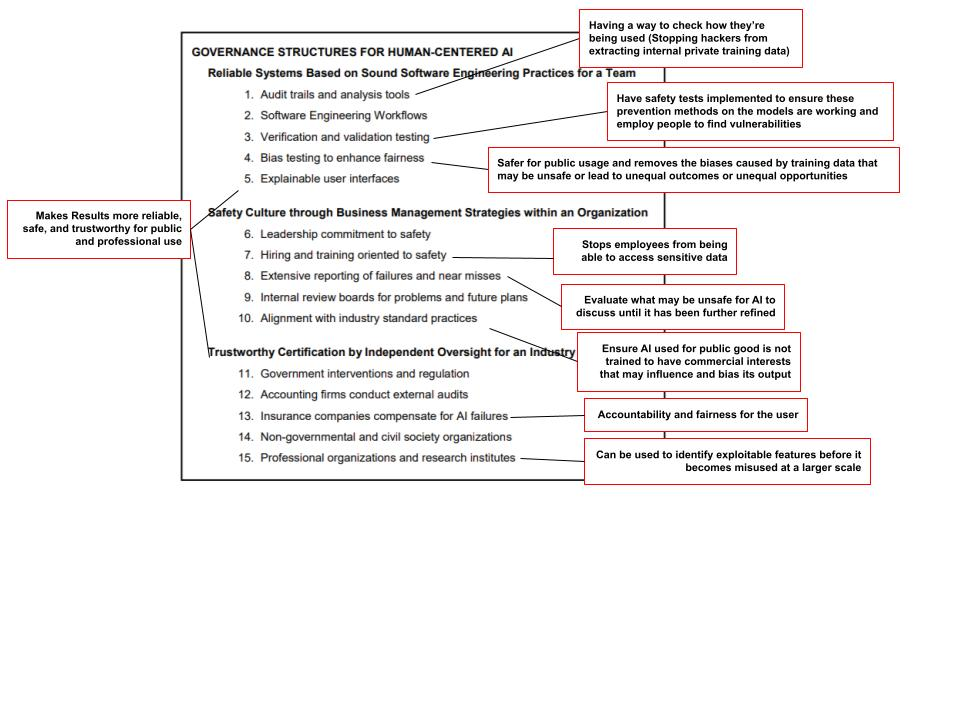
\includegraphics[width=1\linewidth]{aayushbajaj/Documents/uni/comp4920/group-project/report/img/Copy of Shneiderman 2020 - Governance Structures anotated.jpg}
    \caption{Annotated table of Shneiderman's Recommendations for HCAI Systems for Teams, Organisations, and Industry Leaders}
\end{figure}

\subsection{What we learned from this investigation}

Moving from GPT-3 to ChatGPT, despite improvements, there is a fundamental need for better governance to address other issues of safety, privacy and reliability. Furthermore we can see that AI itself will always have an unresolvable problem of bias and we must consider the lack of \textbf{control} that HCAI technologies should have as a risk when comparing it to the potential reward. 

